\chapter{Exercise 3}

\section{Implementation and thoughts behind}
\label{sec:detail_impl_analysisrunner}
In this section a detailed look into the chosen implementation.

\section{UML class diagrams}
\label{sec:class_diagram}
This section shows the the UML class diagramm for measuring the data in the data\_long.dat file. The whole code can be seen at \ref{sec:appendix_analysisrunner}. For a more detailed description of the classes \ref{sec:detail_impl_analysisrunner} is provided.

\begin{landscape}
    \begin{figure}
        \begin{center}
            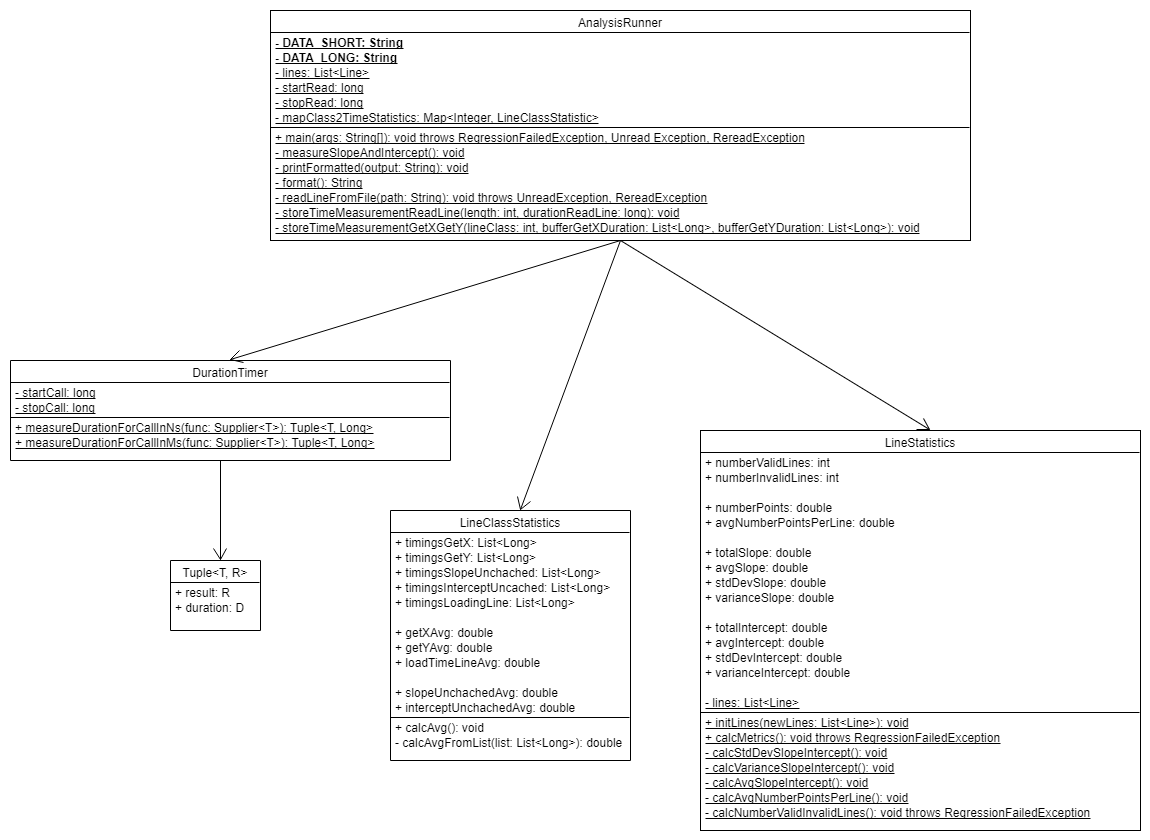
\includegraphics[width=1.60\textwidth]{img/classdiagram.png}
            \caption{UML class diagramm to measure timings}
        \end{center}
    \end{figure}
\end{landscape}

\section{UML sequence diagrams}
\label{sec:seq_diagrams}
In this section UML sequence diagrams are provided for measuring and calculating the wanted statistics. The diagrams are splitted into methods to be more readable. In the end a single UML sequence diagram is provided that references all other provided diagrams. Also for each sequence diagram a small discription is provided and some implementation details are explained.

\subsection{Read lines from file}
The following section describes how the lines within the provided data.dat file are read and how the provided lineReader.jar is used to iterate through the file. This is especially interessting as the time needed to read in the file was measured and is analysed in \ref{chap:4}. For this the implemented DurationTimer was used (see \ref{lst:timingGetX}). It timestamps the start time, executes a given function, timestamps its ends and calculates the duration it took to execute the function. This is then returned as a tuple consisting of the result of the function and the measured duration. As seen in the provided code this is done by supplying the \lstinline[language=java]{Supplier<T> func} parameter, which is then called by the DurationTimer. This can also be seen in the provided sequence diagram (see \ref{fig:seq_read}).

\begin{lstlisting}[language=java, caption=Time measurement for getX with Supplier pattern, label=lst:timingGetX]
    Tuple<Double, Long> timingGetX = DurationTimer.measuredurationForCallInMs(() -> reader.getX());
\end{lstlisting}

\begin{landscape}
    \begin{figure}
        \begin{center}
            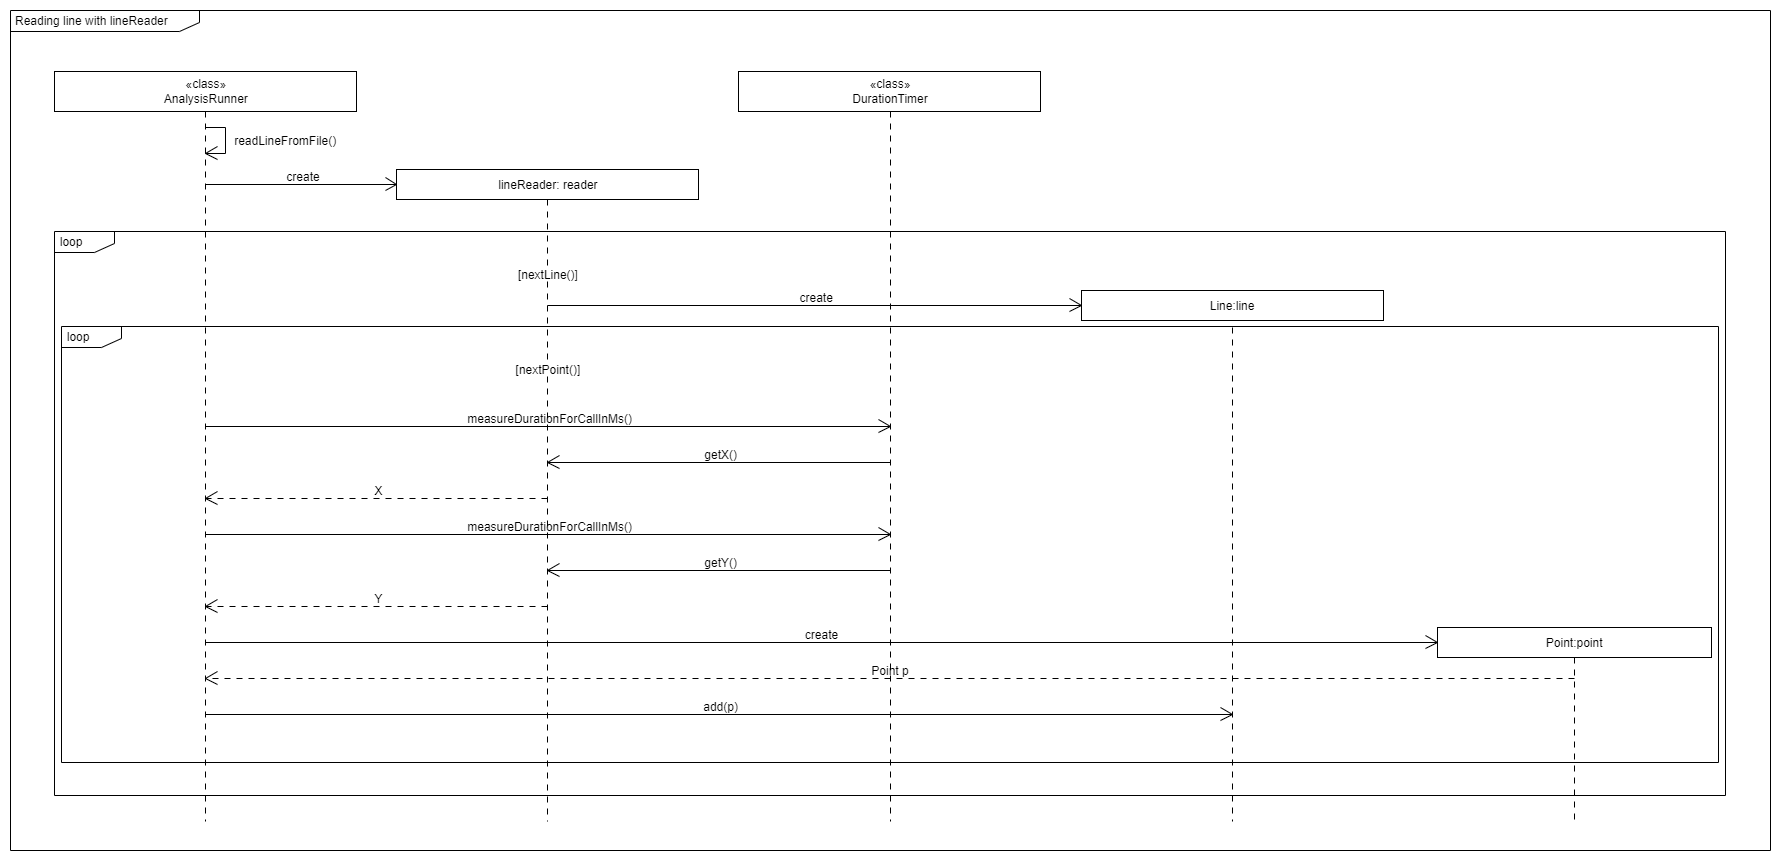
\includegraphics[width=1.75\textwidth, height=0.99\textheight]{img/sequence_read.png}
            \caption{UML sequence diagram for reading in all line in provided data file}
            \label{fig:seq_read}
        \end{center}
    \end{figure}
\end{landscape}
